% !TEX root = template.tex

%----------------------------------------------------------------------
\section{Description / Strategy}

A Skiplist is basically a collection of sorted list nodes, where each node has a link to one or more following nodes. These links form shortcuts which can be used to speed up the searching by skipping one or more nodes. In contrast to tree-based search structures randomized Skiplists don't require re-balancing, thus making the concurrent implementation easier.\\

\noindent The links are arranged in multiple levels. Level $0$ is basically a linked-list of all inserted nodes sorted by value. The higher the level, the less nodes are interconnected meaning that the expected number of nodes on each level decreases exponentially. At the beginning and at the end of each level the \texttt{head} and \texttt{tail} sentinel nodes are placed. The \texttt{head} node is filled with the smallest and \texttt{tail} node with the biggest possible value. These sentinel nodes avoid some special cases in various Skiplist operations.\\

\noindent Nodes can be found by starting at the maximum level and travel along the nodes of the current level as long as possible, thus exploiting the shortcut links. Whenever the value of the inspected node is bigger than the desired value, the level has to be decreased by one and the lookup can go on further.\\

\noindent The randomized Skiplist uses coin flipping to probabilistically determine the height of a new node. The coin flipping is repeated until head is reached, thus the node will have a height of $h$ with a probability of $\frac{1}{2^h}$. The height of the Skiplist, which is the maximum height of all nodes in the list, is $\mathcal{O}(\log{n})$ with high probability. Given that the \texttt{insert}, \texttt{remove} and \texttt{contains} methods all use the internal \texttt{find} method to search for a node as well as its predecessors and successors, the maximum bounds of these methods is equal to the maximum bound of the \texttt{find} method because the remaing parts of these methods take constant time. Given that \texttt{find} either travels down the levels of a node (bounded by height $\mathcal{O}(\log{n})$) or travels along on the nodes on one level, the \texttt{find} method is bounded by $\mathcal{O}(\log{n})$ with high probability. Thus the \texttt{insert}, \texttt{remove} and \texttt{contains} methods are all bounded by $\mathcal{O}(\log{n})$ with high probability.

%----------------------------------------------------------------------
\section{Implementation}

Each concrete Skiplist implements the \texttt{SkipList<T>} interface shown in Listing \ref{lst:skiplist_interface}, providing methods for inserting, removing and searching of values.

\begin{lstlisting}[language=C++, caption={Skiplist Interface}, label=lst:skiplist_interface]
template <typename T>
class SkipList
{
  public:
    static_assert(std::is_integral<T>::value, 
                  "T must be an integral type");
    
    virtual bool empty() = 0;
    virtual size_type size() = 0;
    virtual bool insert(const_reference value) = 0;
    virtual bool remove(const_reference value) = 0;
    virtual bool contains(const_reference value) = 0;
    virtual void clear() = 0;
};
\end{lstlisting}
\noindent For simplicity all the implementations only support integral types and can only handle unique values, meaning that adding the same value twice will fail on the second time. Additionally each type must have a specified minimum and maximum value, because these values will be used by the \texttt{head} and \texttt{tail} sentinel nodes respectively.


%------------------
\subsection{Sequential}
The sequential Skiplist implements the algorithm described in \cite{Herlihy:2008:AMP:1734069} with two small optimizations. The current maximum level of all inserted nodes is cached so that the unused levels can be skipped immediately. Additionally the next-node pointers are stored in a static array within the node object itself, thus eliminating one indirection which would occur when using a dynamic datastructure such as \texttt{std::vector}, with the small downside that it always allocates \texttt{MaxHeight} next-pointer slots even if some slots are unused.

%------------------
\subsection{Concurrent}
The ConcurrentSkiplist is based on the sequential one and uses a \texttt{std::mutex} to control the concurrent access of multiple threads. The implementation simply forwards all requests to the internal instance of a sequential Skiplist after successfully grabbing the lock, thus serializing the access to the internal sequential Skiplist.

%------------------
\subsection{Lazy}
The LazySkipList was based on the algorithm discussed in \cite{}. Instead of serializing all accesses as in the ConcurrentSkipList, it uses a \texttt{std::mutex} per node to serialize as little as possible.

\subsubsection*{Linearizability}
Additionally to the lock, each node contains two flags: \texttt{marked}, indicating that the node is virtually removed from the list and \texttt{fullyLinked}, which is set when the node is fully linked into the SkipList. These flags determine when a performed action (insert or remove) is visible to the other processes and therefore the moment when either the flag \texttt{marked} or \texttt{fullyLinked} is set to \texttt{true} is the linearization point of the respective method.

\subsubsection*{Memory-Managed Version}
In the standard implementations of the LazySkipList (and the LockFreeSkipList) the memory of nodes which are removed from the list is not deallocated. To fix this flaw, the MMLazySkipList uses \texttt{C++11} reference counted smart pointers to deallocate all removed nodes.

%------------------
\subsection{Lock-Free}
The LockFreeSkipList enables concurrent access without locks by using atomic \texttt{compareAndSet} operations for all list manipulations. Any list manipulations in the algorithm consists of changing the successor reference of a node while ensuring that the marked flag \textbf{and} the successor have not changed before. Because standard \texttt{compareAndSet} implementations only support to compare one value, we merge the reference and the marked flag into one \texttt{std::atomic\_uintptr\_t} by using one unused bit of the reference for our marked flag (See Listing \ref{lst:atomic_markable_reference}).

\begin{lstlisting}[language=C++, caption={AtomicMarkableReference}, label=lst:atomic_markable_reference]
template <typename T>
class AtomicMarkableReference
{
  public:
    AtomicMarkableReference(T* ref = nullptr, bool marked = false)
    {
        value = ((uintptr_t)ref & ~mask) | (marked ? 1 : 0);
    }

    T* get(bool& marked)
    {
        uintptr_t tmp = value;
        marked = (bool)(tmp & mask);
        return (T*)(tmp & ~mask);
    }

    bool compareAndSet(T* oldRef, T* newRef, bool oldMarked, bool newMarked)
    {
        uintptr_t oldValue = ((uintptr_t)oldRef & ~mask) | (oldMarked ? 1 : 0);
        uintptr_t newValue = ((uintptr_t)newRef & ~mask) | (newMarked ? 1 : 0);
        return value.compare_exchange_strong(oldValue, newValue);
    }

  private:
    std::atomic_uintptr_t value;
    static const uintptr_t mask = 1;
};
\end{lstlisting}

\subsubsection*{Linearizability}
\noindent As in the LazySkipList the linearization point for removing a list element is the moment when the marked flag is set to \texttt{true}. The linearization point for the insert operation is defined in the LockFreeSkipList as the moment the node is linked in at the bottom level.

%----------------------------------------------------------------------
\section{Experimental Setup}

\subsection{Saturn} \label{subsec:saturn}
Saturn is a shared memory parallel computer with 48 AMD CPU cores.

\begin{table}[H]
  \caption{Hard- and software configuration of Saturn}
  \label{tab:saturn} 
  \begin{center}
    \begin{tabular}{ll}
      CPUs & 4 AMD Opteron 6168 (12 cores, 1.9 GHz, 12 MB cache)\\\hline
      Main Memory & 128 GB DDR3-1333 (currently only 120 GB available)\\\hline
      Operating system & Debian 4.7.6-1 (2016-10-07) x86-64 GNU/Linux\\\hline
      Compiler & gcc (Debian 6.3.0-6) 6.3.0 20170205
    \end{tabular}
  \end{center}
\end{table}

\noindent The hard- and software configuration of the test machine can be seen in Table \ref{tab:saturn}. As compiler options we used \verb|-O3|. We enabled \verb|-DNDEBUG| and \verb|-DCOLLECT_STATISTICS| while performing the benchmarks.

%------------------
\subsection{Simulated Workloads}

Various different workloads have been implemented to simulate different insert, remove and search uses. All the workloads support strong and weak scaling. By using strong scaling the number of items per thread will decrease when the number of threads is increased. By using weak scaling the number of items per thread will always be the same independent of the number of threads. Listing \ref{lst:itemsPerThread} shows the algorithm to determine the number of items per thread used in each workload.

\begin{lstlisting}[language=C++, caption={Items Per Thread depending on the Scaling Mode}, label=lst:itemsPerThread]
static long itemsPerThread(const BaseBenchmarkConfiguration& config)
{
    switch (config.scalingMode) {
    case Scaling::Weak:
        return config.numberOfItems;
    case Scaling::Strong:
        return config.numberOfItems / config.numberOfThreads;
    }
}
\end{lstlisting}

\subsubsection{Interleaving Insert}

The workload shown in Listing \ref{lst:interleaving_insert} simulates the insertion of interleaving values by multiple threads, causing that the predecessor and successor nodes of a node inserted by the current thread are always inserted by other threads. This benchmarks stresses the lazy and lock-free implementations by exploiting the \texttt{fullyLinked} property. 

\begin{lstlisting}[language=C++, caption={Interleaving Insert Workload}, label=lst:interleaving_insert]
const auto items = itemsPerThread(config);
long number = config.initialNumberOfItems + threadId;
for (long i = 0; i < items; i++) {
    list.insert(number);
    number += items;
}
\end{lstlisting}


\subsubsection{Interleaving Remove}

The list will be prefilled with \textit{ItemsPerThread} $*$ \textit{NumberOfThreads} items. The workload shown in Listing \ref{lst:interleaving_remove} simulates the removal of interleaving values by multiple threads, causing that the predecessor and successor nodes of a node removed by the current thread are always removed by other threads. This benchmarks stresses the lazy and lock-free implementations by exploiting the \texttt{marked} property. 

\begin{lstlisting}[language=C++, caption={Interleaving Remove Workload}, label=lst:interleaving_remove]
const auto items = itemsPerThread(config);
long number = threadId;
for (long i = 0; i < items; i++) {
    list.remove(number);
    number += items;
}
\end{lstlisting}


\subsubsection{Mix of Insertions, Removals and Searches}

This workload precomputes random numbers which are uniformly distributed between $0$ and \textit{ItemsPerThread} $*$ \textit{NumberOfThreads}. These random numbers will be passed on to the different Skiplist operations when invoking the work function. Each thread does either insert, remove or search for items. The number of inserting, removing and search threads can be varied when creating the workload.


%------------------
\subsection{Skiplist Statistics}
To get a better picture about the performance and behavior of the Skiplist, performance counters have been added to the \texttt{insert}, \texttt{remove} and \texttt{contains} methods of all Skiplist implementations. These performance counters collect the number of retries, which is especially interesting for the lazy and lock free implementations, as well as the number of successful and failed invocations. Based on these performance counters multiple different metrics can be evaluated, such as the average number of retries of \texttt{insert}, \texttt{remove} and \texttt{contains}.\\

\noindent To minimize the possible influences on the benchmarking results, each thread collects the data in a thread-local statistics object, thus no locking and no atomics are required. At the end of each benchmark the thread-local statistics are aggregated by the benchmark suite to get the complete statistics.\\

\noindent The statistics collection can be completely turned off and thus doesn't add any overhead to production use.

%----------------------------------------------------------------------
\section{Experimental Results}

Each benchmark was repeated $30$ times and the error bars of each plot show the $95\%$ confidence interval. Each benchmark started with an empty list and inserted and/or removed $1000000$ items. Strong scaling was used during benchmarking, thus the number of processed items didn't change with the number of threads. The maximum Skiplist height was $16$. The benchmarks were performed using $1$, $2$, $4$, $8$, $12$, $16$, $24$, $32$, $40$ and $48$ threads. The execution time and Skiplist statistics of each repetition was collected and post-processed.

\subsection{Throughput}

\begin{figure}[H]
    \centering
    
    \begin{subfigure}[b]{0.49\textwidth}
        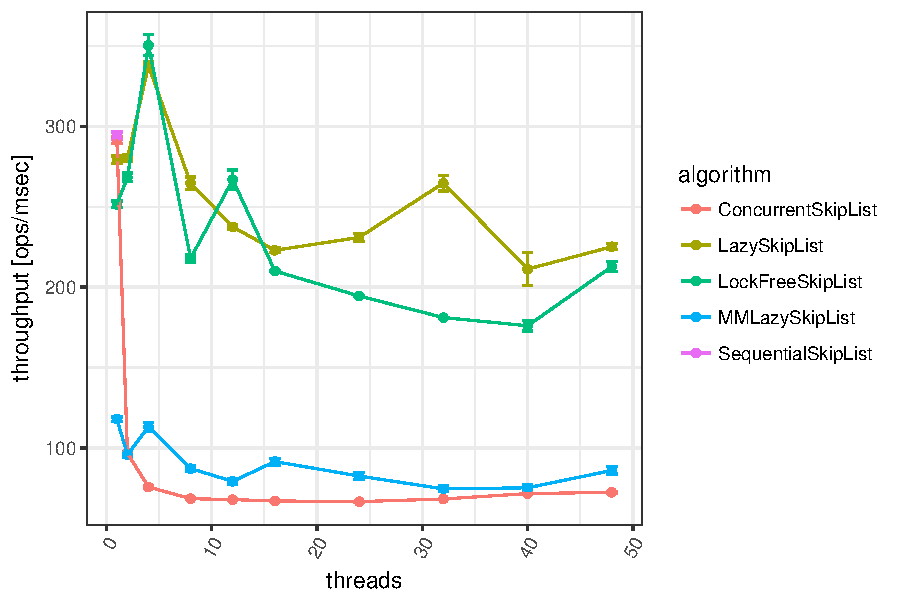
\includegraphics[width=\textwidth]{../plots/interleaving_insert_-_no_failed_inserts_strong_0.pdf}
        \caption{Interleaving Insert}
    \end{subfigure}
    \begin{subfigure}[b]{0.49\textwidth}
        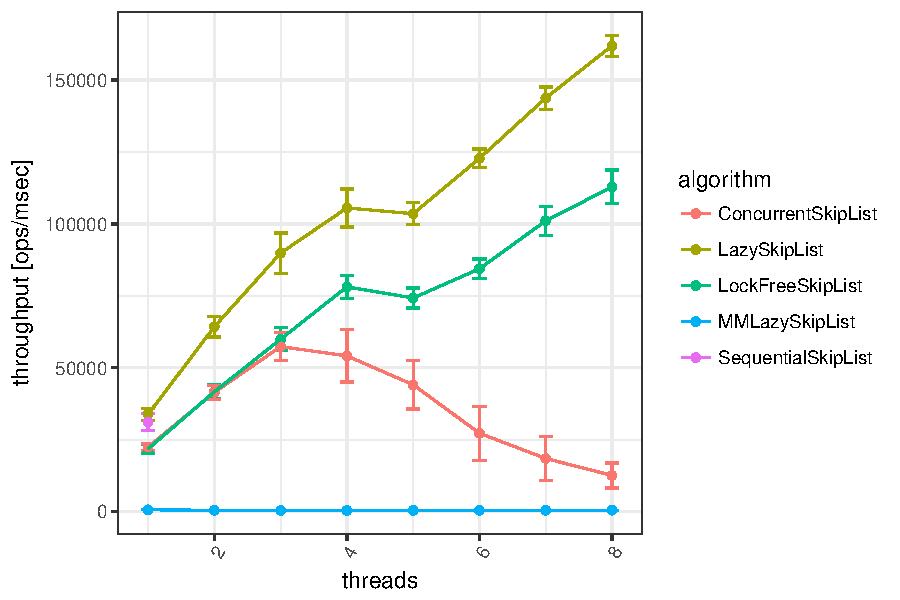
\includegraphics[width=\textwidth]{../plots/interleaving_remove_-_no_failed_removes_strong_0.pdf}
        \caption{Interleaving Remove}
    \end{subfigure}
    
    \begin{subfigure}[b]{0.49\textwidth}
        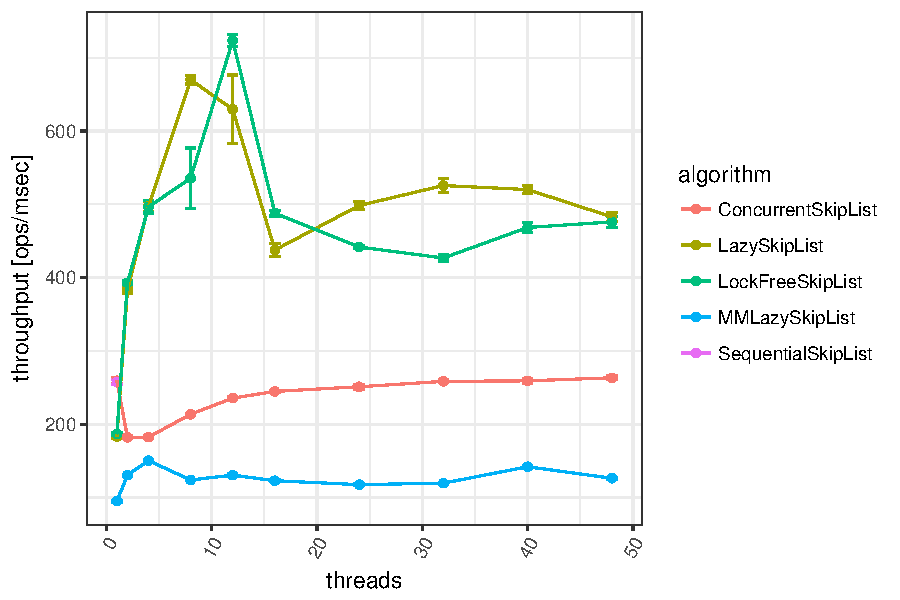
\includegraphics[width=\textwidth]{../plots/mixed_workload_-_50p_insert_,_20p_remove_,_30p_search_strong_0.pdf}
        \caption{50\% Insert, 20\% Remove, 30\% Contains}
    \end{subfigure}
    \begin{subfigure}[b]{0.49\textwidth}
        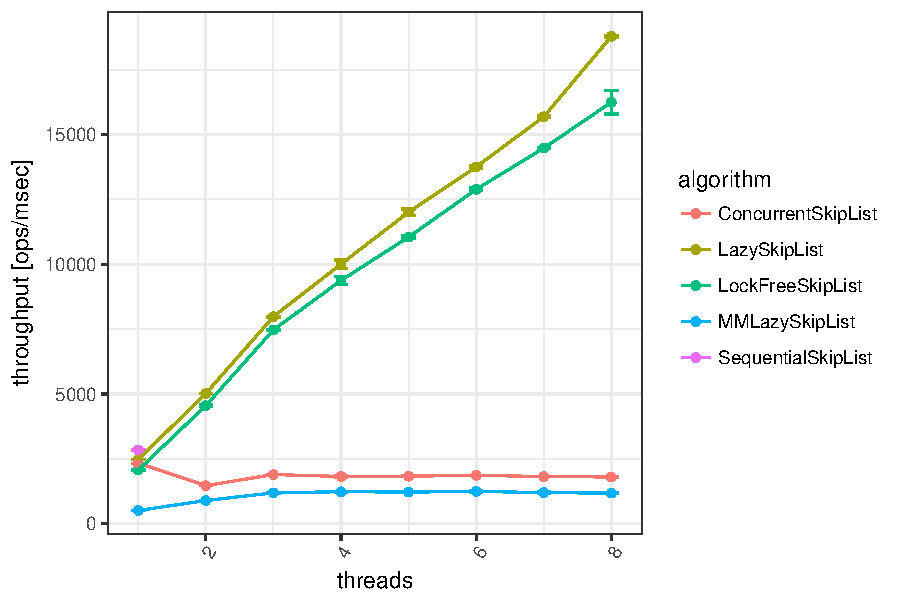
\includegraphics[width=\textwidth]{../plots/mixed_workload_-_70p_insert_,_30p_remove_strong_0.pdf}
        \caption{70\% Insert, 30\% Remove}
    \end{subfigure}
    
    \caption{SkipList Throughput of Different Algorithms under Different Workloads}
\end{figure}


\subsection{Performance Counters}

\subsubsection*{Interleaving Insert/Remove}

\begin{figure}[H]
    \centering
    
    \begin{subfigure}[b]{0.49\textwidth}
        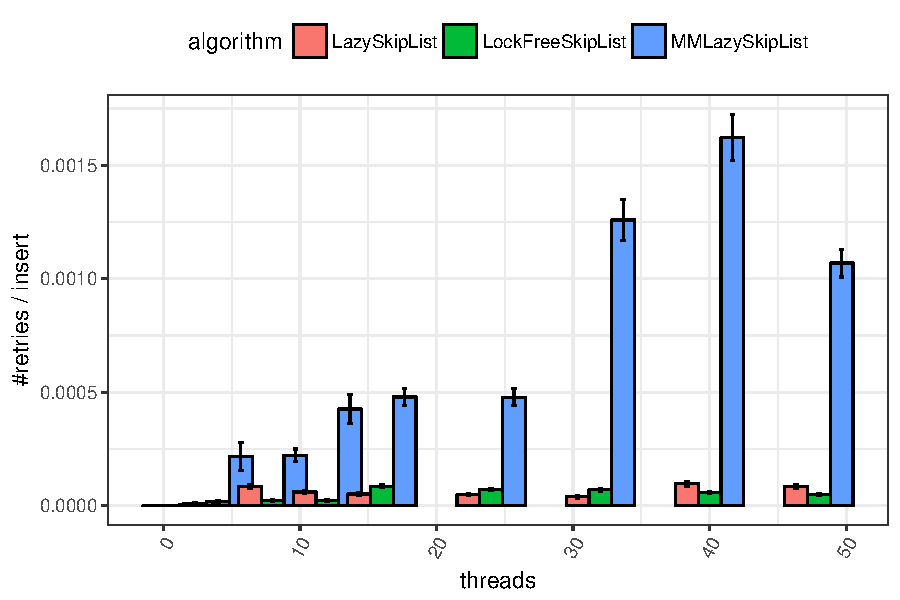
\includegraphics[width=\textwidth]{../plots/insert_retries_interleaving_insert_-_no_failed_inserts_strong_0.pdf}
        \caption{\#Retries per Insert}
    \end{subfigure}
    \begin{subfigure}[b]{0.49\textwidth}
        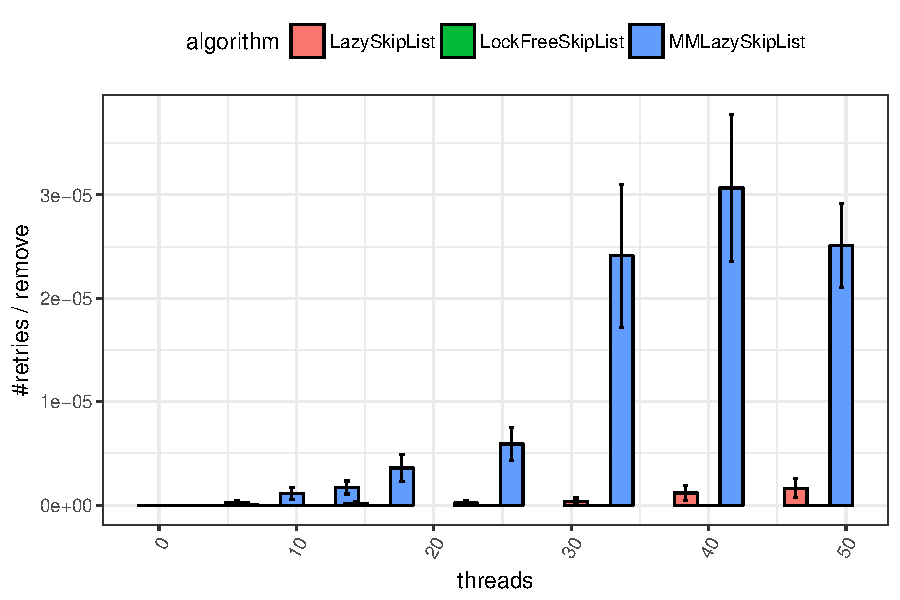
\includegraphics[width=\textwidth]{../plots/remove_retries_interleaving_remove_-_no_failed_removes_strong_0.pdf}
        \caption{\#Retries per Remove}
    \end{subfigure}
\end{figure} 


\subsubsection*{50\% Insert, 20\% Remove, 30\% Contains}

\begin{figure}[H]
    \centering
    \begin{subfigure}[b]{0.49\textwidth}
        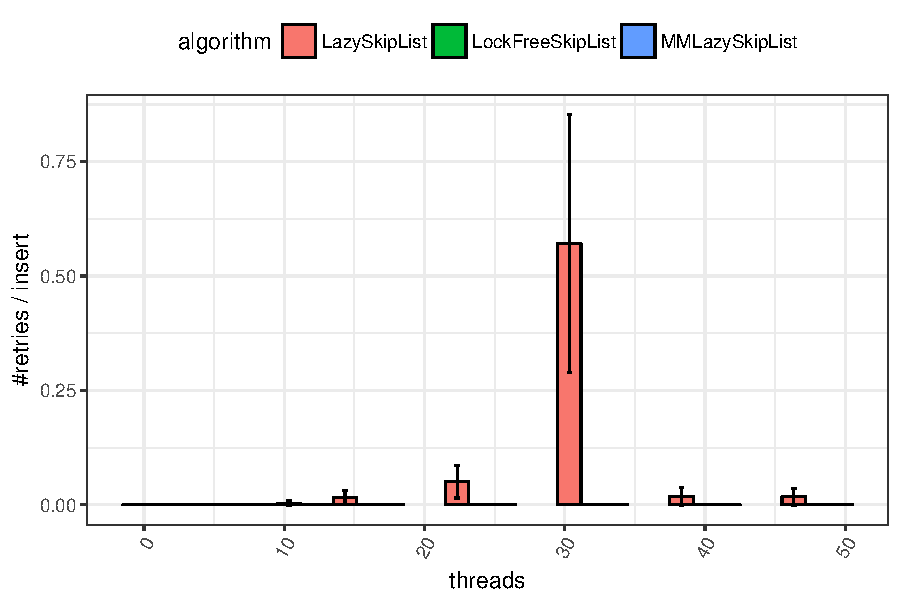
\includegraphics[width=\textwidth]{../plots/insert_retries_mixed_workload_-_50p_insert_,_20p_remove_,_30p_search_strong_0.pdf}
        \caption{\#Retries per Insert}
    \end{subfigure}
    \begin{subfigure}[b]{0.49\textwidth}
        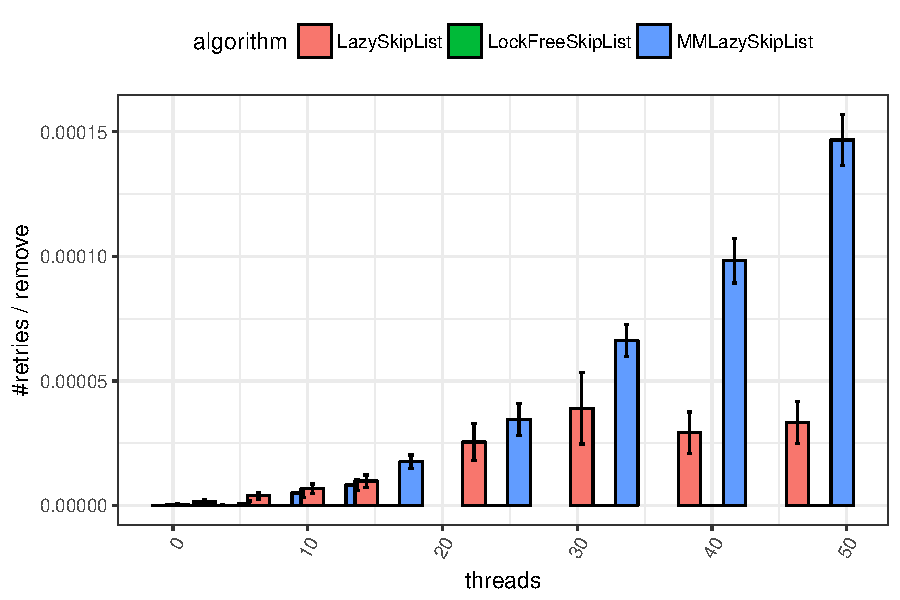
\includegraphics[width=\textwidth]{../plots/remove_retries_mixed_workload_-_50p_insert_,_20p_remove_,_30p_search_strong_0.pdf}
        \caption{\#Retries per Remove}
    \end{subfigure}
\end{figure}

\subsubsection*{70\% Insert, 30\% Remove}

\begin{figure}[H]
    \centering
    \begin{subfigure}[b]{0.49\textwidth}
        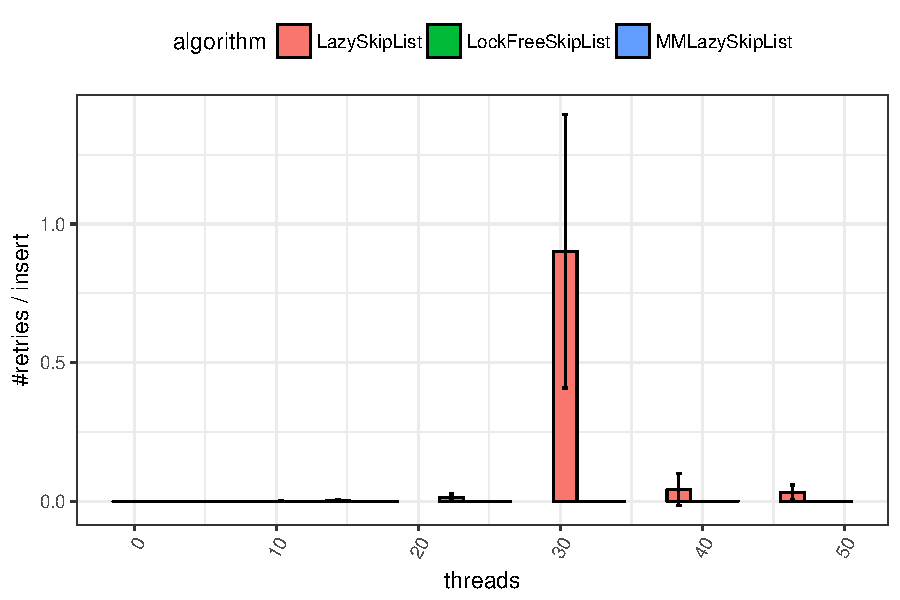
\includegraphics[width=\textwidth]{../plots/insert_retries_mixed_workload_-_70p_insert_,_30p_remove_strong_0.pdf}
        \caption{\#Retries per Insert}
    \end{subfigure}
       \begin{subfigure}[b]{0.49\textwidth}
        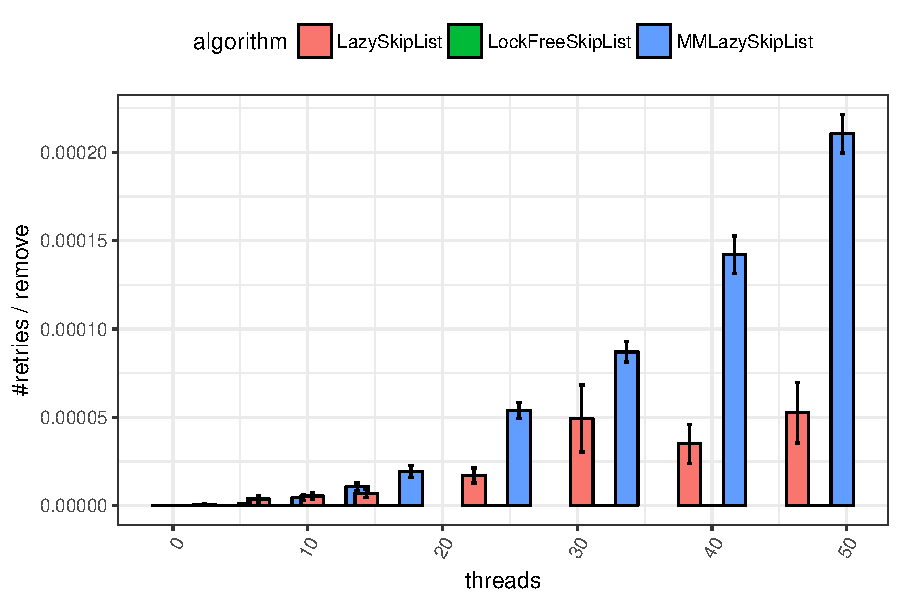
\includegraphics[width=\textwidth]{../plots/remove_retries_mixed_workload_-_70p_insert_,_30p_remove_strong_0.pdf}
        \caption{\#Retries per Remove}
    \end{subfigure}
\end{figure}
